\documentclass[11pt]{beamer}
\usepackage[utf8]{inputenc}
\usepackage[T1]{fontenc}
%\usepackage{natbib}
\usetheme{Pittsburgh}
\usepackage{verbatim} 
\usepackage[english]{babel}
\usepackage{epstopdf}
\usepackage{multicol}
%\titlegraphic{%\vspace*{1cm}
%	\includegraphics[width=2.5cm]{logo_udelar}
	%\hspace*{1cm}~%
%		\includegraphics[width=3.5cm]{logo_FCEA.png}
%}
\setbeamertemplate{navigation symbols}{}
\setbeamertemplate{footline}[frame number]
\AtBeginSection{ 
	\begin{frame}
		\frametitle{Index}
			\tableofcontents[currentsection]
	\end{frame}
}
\begin{document}
	\title{Modelos dinámicos y computacionales en Economía}
	\subtitle{Modelos Basados en Agentes: Distribución}
	%\logo{}
	\institute{Licenciatura en Economía, FCEA, UDELAR}
	\date{9 de noviembre de 2023}

	%\subject{}
	%\setbeamercovered{transparent}
	%\setbeamertemplate{navigation symbols}{}
	\frame[plain]{
	\begin{figure}
	\centering
	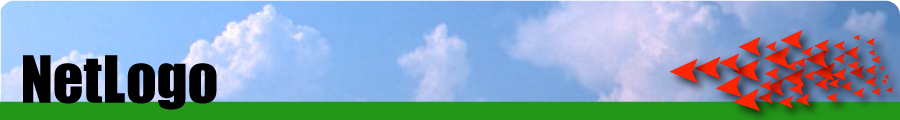
\includegraphics[width=0.7\linewidth]{figuras/netlogo-title-wide-60}
	%		\caption{}
	\label{fig:netlogo-title-wide-60}
\end{figure}	
		\vspace{-1cm}
\maketitle
}
%\setbeamertemplate{background}{\includegraphics[width=2 cm]{logo_FCEA.png}}

\begin{frame}
\frametitle{Contenido de la clase:}
\begin{itemize}
	\item Problema de la distribución del ingreso en Economía
    \item Distribuciones en los sistemas económicos
	\item Ejemplo: Un modelo simple de intercambio
\end{itemize}
\end{frame}

\begin{frame}
	\frametitle{Distribución del ingreso en Economía}
	\framesubtitle{Reduccionismo}
	\begin{itemize}
		\item Un ejemplo clásico: ¿cómo estudiamos la distribución en modelos con un individuo (o \textit{n individuos iguales})?
		\item Problema: la naturaleza del fenómeno a analizar.
		\item ¿Cuáles son las causas de la desigualdad?
		\item ¿Existen patrones o regularidades empíricas y estadísticas comunes a la distribución del ingreso en diferentes sociedades y distintos momentos del tiempo?
		\item Pareto (1906): una fracción pequeña de la sociedad controla una alta proporción de la riqueza.
	\end{itemize}
\end{frame}

\begin{frame}
\frametitle{Distribución del ingreso en Economía}
\framesubtitle{Ley de Pareto}
\begin{itemize}
	\item Se utilizan los términos distribución de potencia (\textit{power law}) y ley de Pareto para describir eventos tales como:
	\begin{itemize}
		\item hay pocas ciudades ``grandes'' y muchas ciudades ``pequeñas''.
		\item Pocas palabras que se utilizan con mucha frecuencia, mientras que muchas se utilizan pocas veces.
		\item Son pocos los grandes terremotos (según la escala de Richter) pero son muchos los movimientos de baja intensidad.
	\end{itemize}
	\item Como observó Pareto, la distribución del ingreso sigue una \textit{power law}, con un 80\% de los ingresos en manos del 20\% más rico (regla 80/20).
\end{itemize}
\end{frame}

\begin{frame}
\frametitle{Distribución del ingreso en Economía}
\framesubtitle{Evolución de la distribución del ingreso en EE.UU. para el top 1\% y el top 0.1\%. Fuente: Piketty et al. (2018)\footnote{\scriptsize{Piketty, T., Saez, E., \& Zucman, G. (2018). Distributional national accounts: methods and estimates for the United States. \textit{The Quarterly Journal of Economics, 133}(2), 553-609.}}}

\begin{figure}
	\centering
	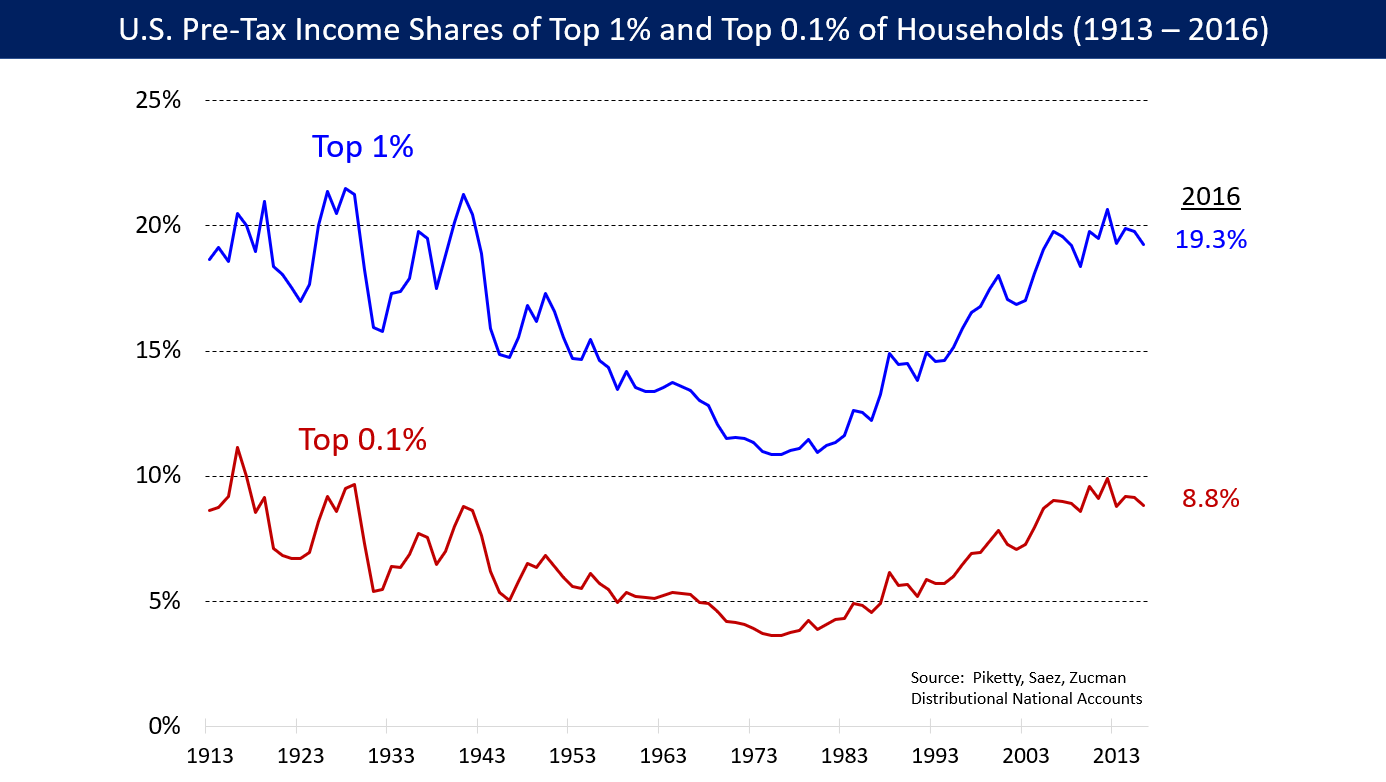
\includegraphics[width=0.8\linewidth]{figuras/US_income_share}
\label{fig:usincomeshare}
\end{figure}

\end{frame}

\begin{frame}
\frametitle{Distribución del ingreso en Economía}
\framesubtitle{Ley de Pareto (cont.)}
Función de distribución:
\begin{equation*}
p(x)=Ax^{-\alpha}
\end{equation*}
Si tomamos logaritmos, esta relación puede describirse a partir de una recta con pendiente negativa (e igual a $\alpha$ en valor absoluto):
\begin{equation*}
ln[p(x)]=ln[A] -\alpha ln[x]
\end{equation*}
A partir de la función de distribución acumulada, se puede llegar a la siguiente relación:
\begin{equation*}
W=P^{\frac{2-\alpha}{1-\alpha}}
\end{equation*}
Donde W es la proporción del ingreso en manos de la fracción P más rica.
\begin{itemize}
	\item La relación 80/20 (observada), ¿para qué valor de $\alpha$ se aplica?
	\item ¿Cuál es el valor aproximado de $\alpha$ para EE.UU. en 2016? 
\end{itemize}
\end{frame}

\begin{frame}
\frametitle{Distribución del ingreso en Economía}
\framesubtitle{Evidencia empírica \footnote{\scriptsize{ Clementi, F., \& Gallegati, M. (2005). Pareto’s law of income distribution: Evidence for Germany, the United Kingdom, and the United States. In Econophysics of wealth distributions (pp. 3-14). Springer, Milano.}}}
\begin{figure}
	\centering
	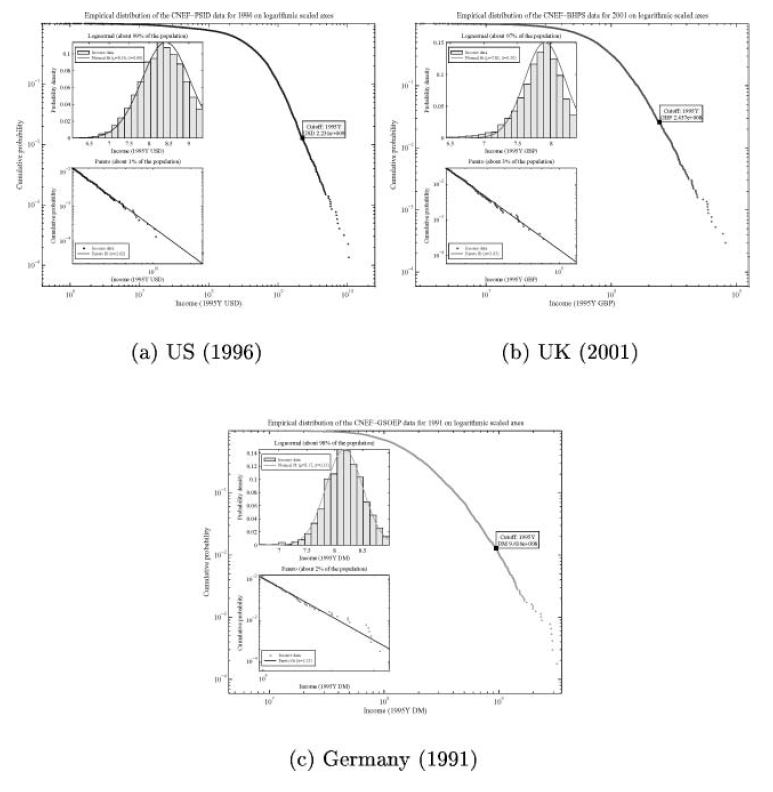
\includegraphics[width=0.55\linewidth]{figuras/inequality_1}
%	\caption{}
	\label{fig:inequality1}
\end{figure}
\end{frame}

\begin{frame}{Leyes de Potencia}
\framesubtitle{Introducción}
\begin{itemize}
    \item En Economía, hay muchas distribuciones que son diferentes a la distribución Normal.
    \item Distribuciones estables: familia de distribuciones que incluye a la distribución Normal.
    \item Fenómenos críticos como generadores de procesos agregados que se distribuyen bajo leyes de escala.
    \item A tomar en cuenta:
    \begin{itemize}
        \item ¿existen valores representativos del conjunto de datos?
        \item ¿qué podemos decir de la incertidumbre?
        \item la presencia de una estructura de interdependencias en los datos, ¿qué consecuencias tiene al momento de hacer inferencia?
        \item ¿cómo podemos analizar la existencia de leyes de escala en un conjunto de datos?
    \end{itemize}
\end{itemize}
\end{frame}

\begin{frame}{Leyes de Potencia}
\framesubtitle{Definiciones}
función de distribución: $p(x)=Ax^{-\alpha}$\\
\vspace{0.5cm}
función de distribución acumulada:
\begin{equation*}
\int_{x_{min}}^{\infty} p(x)dx=\int_{x_{min}}^{\infty}Ax^{-\alpha}dx=\dfrac{A}{1-\alpha}\left[x^{1-\alpha}\right] _{x_{min}}^{\infty}=1
\end{equation*}
Lo cual se cumple si \color{blue} \textbf{$\alpha > 1$ } \color{black}.\\
\vspace{0.5cm}

Primer momento:
\begin{equation*}
\langle x \rangle = \int_{x_{min}}^{\infty} x^{1}p(x)dx=\int_{x_{min}}^{\infty}Ax^{1-\alpha}dx=\dfrac{A}{2-\alpha}\left[x^{2-\alpha}\right] _{x_{min}}^{\infty}
\end{equation*}
...es finito si: \pause \color{blue} \textbf{$\alpha > 2$ } \color{black}
\end{frame}

\begin{frame}{Leyes de Potencia}
\framesubtitle{Definiciones (cont.)}
Segundo momento:
\begin{equation*}
\langle x^{2} \rangle = \int_{x_{min}}^{\infty} x^{2}p(x)dx=\int_{x_{min}}^{\infty}Ax^{2-\alpha}dx=\dfrac{A}{3-\alpha}\left[x^{3-\alpha}\right] _{x_{min}}^{\infty}
\end{equation*}
...es finito si: \pause \color{blue} \textbf{$\alpha > 3$ } \color{black}\\
\vspace{0.3cm}
En general: 
\begin{equation*}
\langle x^{m} \rangle = \int_{x_{min}}^{\infty} x^{m}p(x)dx=\dfrac{\alpha-1}{\alpha - m -1}x^{m}_{min} 
\end{equation*}
por lo cual $\langle x^{m} \rangle$ es finito para $\alpha > m$.\\
\vspace{0.3cm}

¿Momentos infinitos? \pause en la realidad, calculamos los momentos sobre una muestra finita de realizaciones de la variable aleatoria. Son propiedades asintóticas, por lo tanto en la realidad siempre vamos a encontrar valores finitos. 
\end{frame}

\begin{frame}{Leyes de Potencia}
\framesubtitle{Ejemplo con muestra finita}
Alta volatilidad en la variación de precios de los productos: cambios en los precios relativos no captados por el índice general.
\begin{multicols}{2} 
{\small \begin{itemize}
	\item Estos resultados nos indican que a medida que aumenta la cantidad de productos en el índice, la volatilidad del índice aumenta.
	\item En el ejemplo siguiente, se simula el desvío estándar del índice mediante bootstrap, para distintos tamaños del índice (15, 30, 60, 150 productos) y se compara con la serie original.
\end{itemize}}
	\begin{figure}
	\centering
	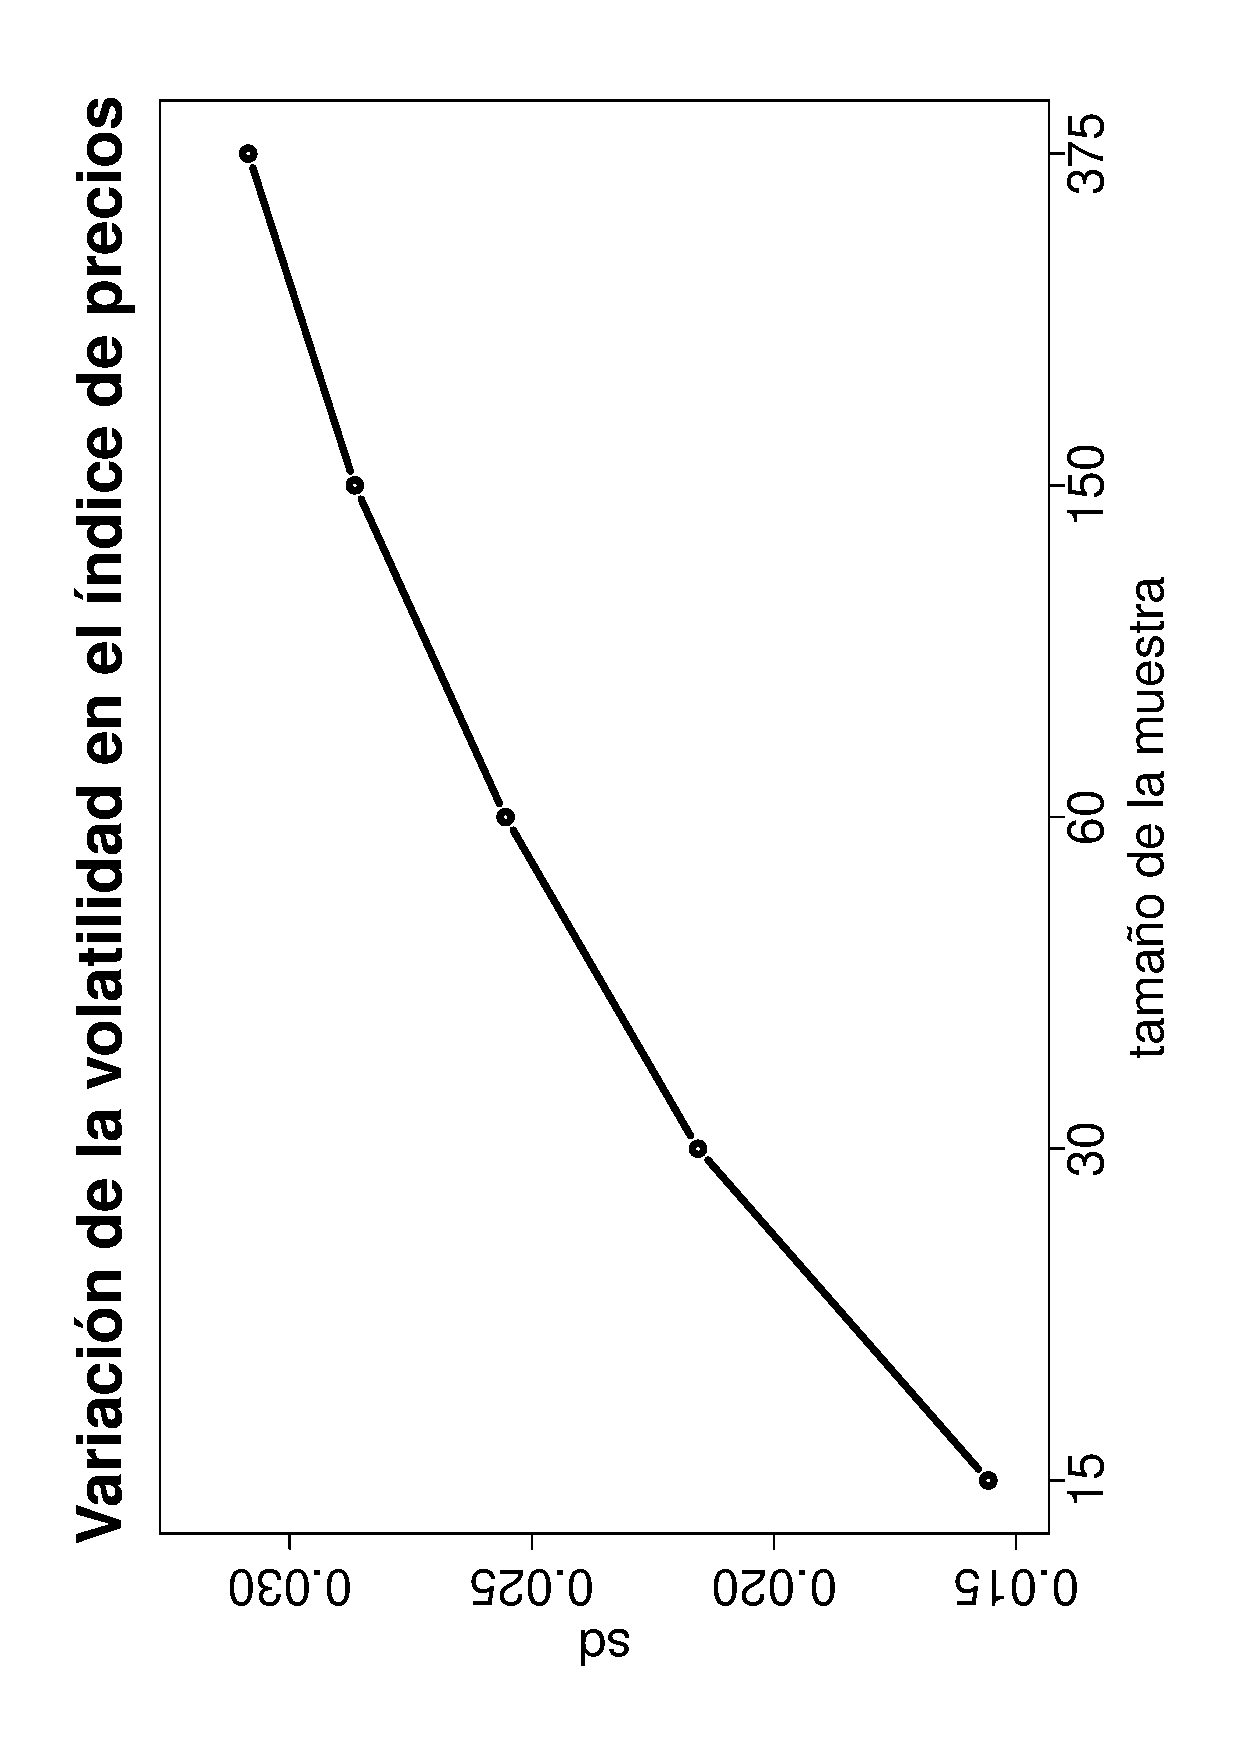
\includegraphics[width=0.60\linewidth,angle=270]{plots01/volatilidad_muestra}
	\caption{{\footnotesize Aumento de la volatilidad de la serie, respecto de la cantidad de productos. Elaboración propia en base a datos del INE, Uruguay.}}
	\label{fig:logexpinfl12}
\end{figure}
\end{multicols}
\end{frame}

\begin{frame}{Leyes de Potencia}
\framesubtitle{Libres de escala}
\begin{itemize}
    \item una distribución $p(x)$ es libre de escala si $p(bx)=g(b)p(x)$,
    \item ejemplo: $p(bx)=A(bx)^{-\alpha}=(Ab^{-\alpha})x^{-\alpha} \longrightarrow p(bx)=Bx^{-\alpha}$, con $B=(Ab^{-\alpha})$
    \item es decir que es proporcional a la distribución original.
    \item por lo cual, este factor $b$ es irrelevante al momento de analizar las propiedades: desaparece al normalizar la distribución.
    \item \textit{Propiedad de universalidad}
\end{itemize}
\begin{table}
\centering
\scriptsize
\begin{tabular}{|c|c|c|}
\hline
	& $x_{min}$ & $\alpha$ \\
	\hline
frecuencia de uso de palabras	& 1 & 2.20 \\
	\hline
número de citas en artículos & 100 & 3.04 \\
	\hline
número de clics en sitios web	& 1  & 2.4 \\
	\hline
llamadas recibidas	& 10 & 2.22 \\
	\hline
magnitud de terremotos	& 3.8 & 3.04 \\
	\hline
diámetro de los cráteres en la Luna	& 0.01 & 3.14 \\
	\hline
intensidad de llamaradas solares & 200 & 1.83 \\
	\hline
frecuencia de nombres & 10000 & 1.94 \\
	\hline
población en ciudades (US)	& 40000 & 2.3 \\
	\hline
\end{tabular}
\end{table}
\end{frame}

\begin{frame}[allowframebreaks]
\frametitle{Leyes de Potencia}
\framesubtitle{Mecanismos para generar leyes de potencia}
\begin{enumerate}
    \item Combinación de exponenciales:\\
    supongamos que $y$ sigue una distribución exponencial; luego, $x$ se distribuye: $x\sim e^{by}$. En este caso, la función de distribución de $x$
sigue una ley de potencias.
\item inversas de cantidades:\\
supongamos que $y$ se distribuye $p(y)$, pero nosotros estamos interesados en su recíproco $x$ ($x=1/y$). Para valores altos de $x$, $p(x)\sim x^{-2}$ \\(en general, para $x=y^{-\gamma}$ tenemos que $p(x)=x^{-\alpha}$, con $\alpha=1+1/\gamma$).
\item Random walks: Gambler’s ruin
\item Procesos de Yule: la distribución de especies en un grupo taxonómico sigue una ley de potencias.
\item Transiciones de fase y fenómenos críticos:\\
\begin{itemize}
    \item En muchos casos los fenómenos macroscópicos tienen un solo estado; sin embargo bajo ciertas circunstancias esto puede cambiar y el sistema pasa a ser libre de escala.
    \item En la vecindad de la transición de fase ocurren fenómenos críticos, entre otros la aparición de leyes de potencia.
    \item ejemplo: \textit{fire model} (modelos de percolación)
\end{itemize} 
\item Criticalidad auto-organizada (SOC):\\
\begin{itemize}
    \item No es casualidad que en tantas ocasiones ocurran este tipo de fenómenos críticos.
    \item Bak et al. (1987): los sistemas se auto-organizan para ir hacia ese estado crítico.
    \item Ejemplo: \textit{modelo de la pila de arena}.
\end{itemize}
\end{enumerate}

\end{frame}

\begin{frame}
\frametitle{Un modelo simple de intercambio\footnote{ \scriptsize{Dragulescu, A., \& Yakovenko, V. M. (2000). Statistical mechanics of money. \textit{The European Physical Journal B-Condensed Matter and Complex Systems, 17}(4), 723-729.}}}
En este caso, analizaremos un modelo muy simple de intercambio:
\begin{itemize}
	\item Supongamos que tenemos un mundo con 500 individuos, cada uno con \$100 de riqueza inicial.
	\item En cada tick del reloj, se le entrega \$1 a otra persona \textit{al azar}.
	\item En este modelo, la cantidad de dinero permanece fija y no podemos pedir prestado. 
\end{itemize}
\underline{Preguntas:}
\begin{itemize}
	\item ¿Qué ocurrirá con la distribución del dinero, luego de 10000 períodos? 
	\item ¿La riqueza se concentrará en unas pocas manos o será distribuida equitativamente?
\end{itemize}
\end{frame}

\begin{frame}
\frametitle{Un modelo simple de intercambio (cont.)}
\begin{itemize}
	\item En \textbf{Archivo / Biblioteca de Modelos / IABM Textbook / chapter 2 / "Simple Economy"}
	\item Chequear:
	\begin{itemize}
		\item ¿cuántos tipos de agentes tenemos en este modelo?
		\item ¿qué variables son específicas de estos agentes? 
		\item ¿cuáles son las variables globales?
		\item ¿qué procedimientos hay en este modelo?
	\end{itemize}
\end{itemize}	
\end{frame}

\begin{frame}
\frametitle{Un modelo simple de intercambio (cont.)}
\begin{itemize}
\item No hay variables globales. Hay algunos parámetros ya incluidos en el código.
\item Tipos de agentes: sólo turtles (hogares en este caso).
\item Variable específica: \textbf{wealth}.
\item Procedimientos: \textbf{SETUP}, \textbf{GO}, \textbf{TRANSACT}.
\end{itemize}	
\end{frame}

\begin{frame}
\frametitle{Un modelo simple de intercambio (cont.)}
\underline{Ejercicio 1:}
\begin{itemize}
	\item ¿Qué ocurrirá con la distribución del dinero, luego de 10000 períodos? 
	\item ¿La riqueza se concentrará en unas pocas manos o será distribuida equitativamente?
\end{itemize}
\underline{Ejercicio 2:}
\begin{itemize}
	\item Modificar la cantidad de agentes (aumentar a 1000). 
	\item Dar la posibilidad de endeudarse (hasta un tope de \$20).
	\item Modificar la cantidad de dinero a transferir:
	\begin{itemize}
		\item una cantidad fija > 1
		\item una cantidad aleatoria: $U \sim [0; 2]$
	\end{itemize}
\end{itemize}
\end{frame}

\begin{frame}
\frametitle{Un modelo simple de intercambio (cont.)}
\framesubtitle{Algunos resultados}
\begin{itemize}
	\item La distribución resultante no es Gaussiana.
	\item Pertenece a una amplia clase de modelos donde una cantidad fija es intercambiada en un sistema cerrado.
	\item Distribución de Boltzmann: para un sistema de estas características, se encuentra que la distribución final es del tipo exponencial.
	\item Este tipo de distribuciones son comunes en la \textit{mecánica estadística}, que utiliza la teoría de la probabilidad para analizar el comportamiento termodinámico de sistemas con gran cantidad de partículas. 
\end{itemize}
\end{frame}

\begin{frame}
\frametitle{Un modelo simple de intercambio (cont.)}
\framesubtitle{Algunos resultados}
¿Qué sucede cuando permitimos que los agentes se endeuden?

\begin{columns}
\begin{column}{0.5\linewidth}
\begin{itemize}
	\item En este caso, la distribución resultante sigue siendo exponencial. 
	\item La diferencia radica en que existe una mayor desigualdad.
	\item Esto sucede porque sigue siendo un sistema cerrado. Si asumimos que la riqueza puede acumularse, crearse o destruirse, entonces la distribución resultante es una \textit{power law}.
\end{itemize}
\end{column}
\begin{column}{0.5\linewidth}
\begin{figure}
	\centering
	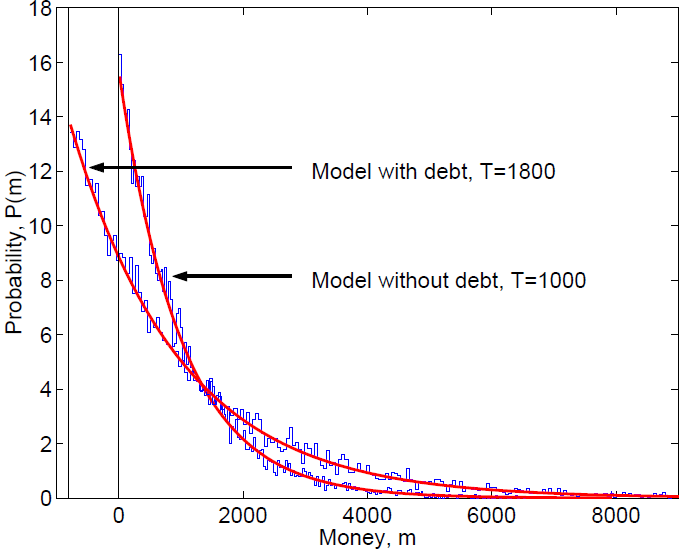
\includegraphics[width=0.85\linewidth]{figuras/inequality_2.png}
	\caption{{\scriptsize Distribución del ingreso con y sin posibilidades de endeudameinto. Fuente: Dragulescu \& Yakovenko (2000).}}
	\label{fig:inequality1}
\end{figure}

\end{column}
\end{columns}
\end{frame}
\end{document}
